
\documentclass[12pt]{article}
\usepackage{enumitem}
\usepackage{geometry}
\usepackage{graphicx}
\geometry{margin=1in}

\title{TestRail Report – Snapshot 2}
\author{Haonan Ma}
\date{}

\begin{document}

\maketitle

\section*{Overview}
This document contains the functional and security test cases implemented and verified during Snapshot 2 of the LAPD1 Transcript Analysis System project.

\section*{Snapshot Summary Image}
\begin{center}
    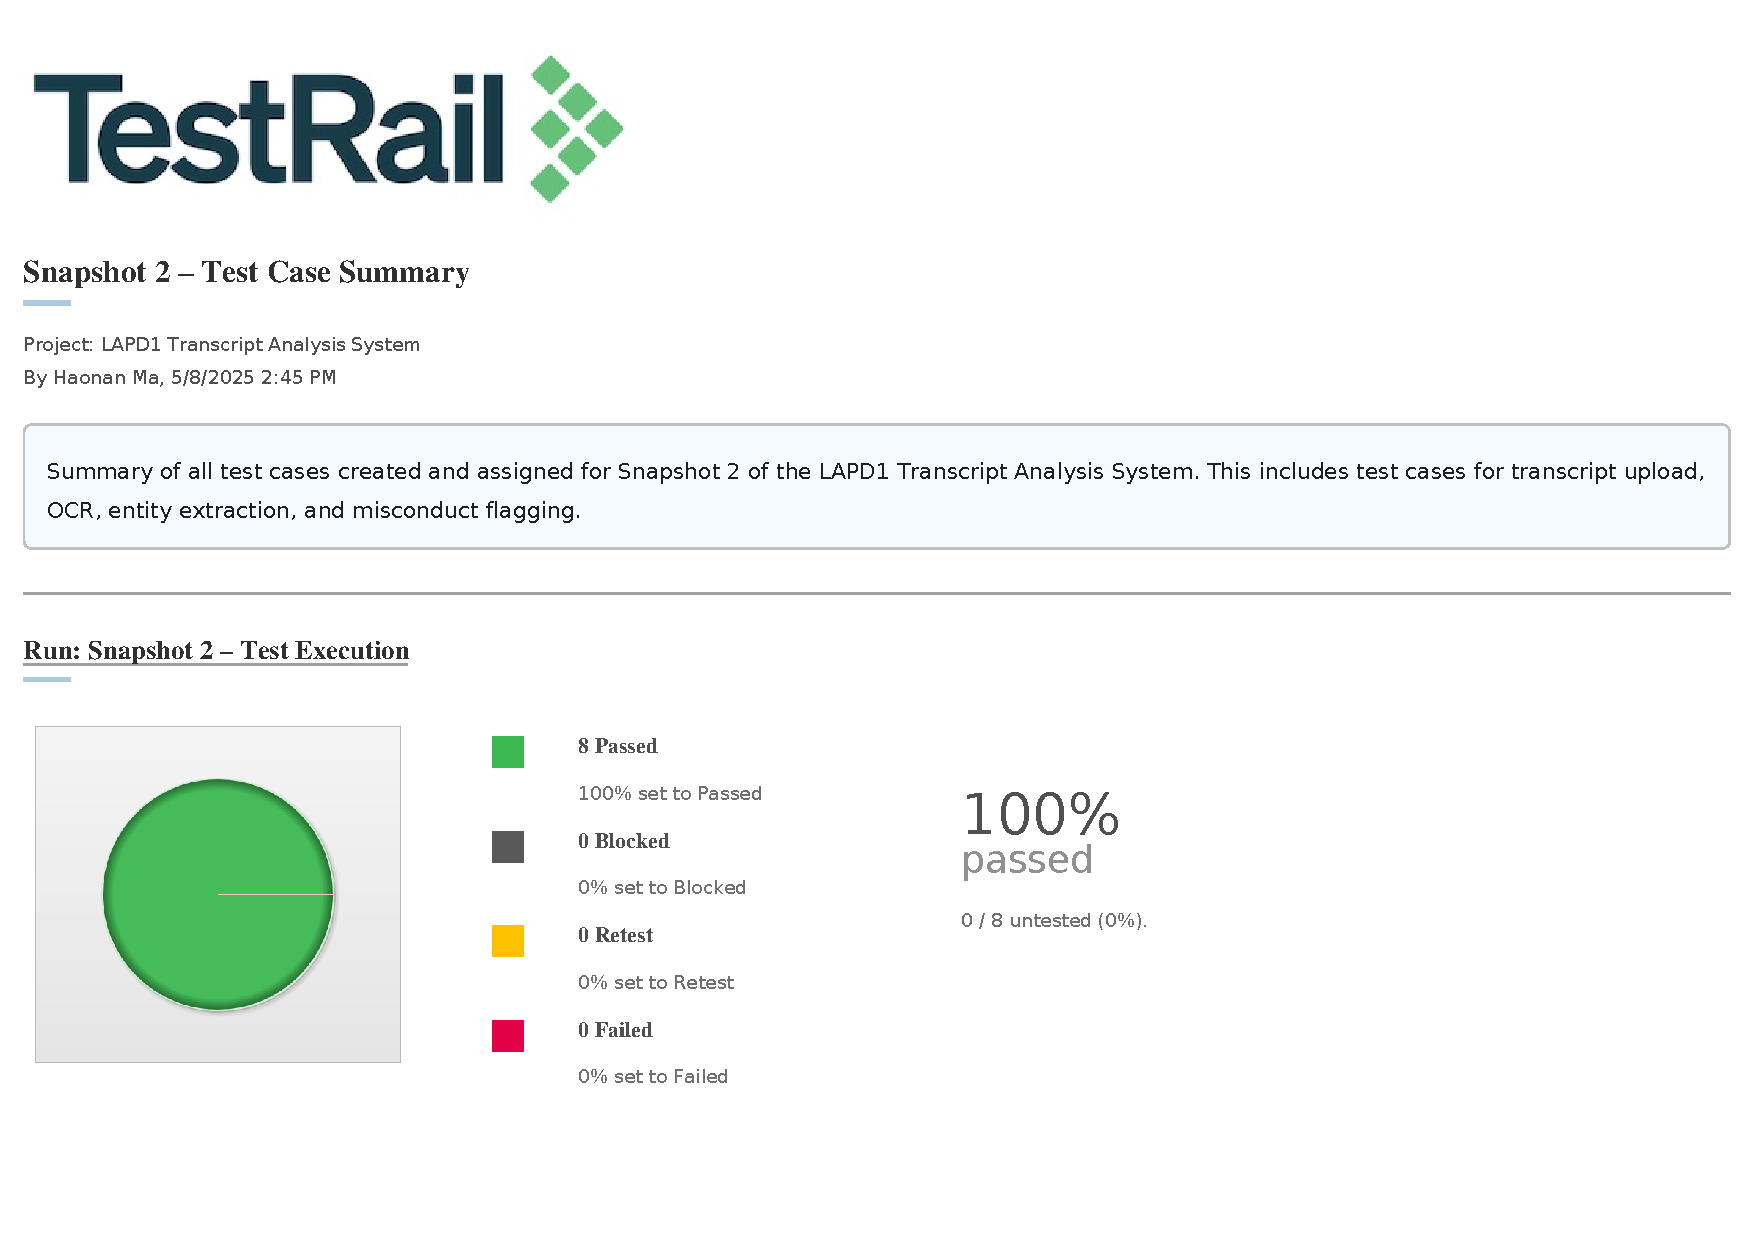
\includegraphics[width=\textwidth]{snapshot2image}
\end{center}

\section*{Test Cases}

\subsection*{Test Case 1: Upload Valid Transcript File}
\textbf{Type:} Functional \\
\textbf{Priority:} Medium \\
\textbf{Estimate:} 5m \\
\textbf{Preconditions:} User is logged in and is on the upload page. \\
\textbf{Steps:}
\begin{enumerate}[label=\arabic*.]
\item Click the “Choose File” button.
\item Select a valid .pdf transcript file.
\item Click the “Analyze” button.
\end{enumerate}
\textbf{Expected Result:} The file is uploaded successfully, and the system transitions to the analysis page with a confirmation message.

\subsection*{Test Case 2: Upload Scanned PDF and Trigger OCR}
\textbf{Type:} Functional \\
\textbf{Priority:} Medium \\
\textbf{Estimate:} 5m \\
\textbf{Preconditions:} User is logged in and is on the upload page. \\
\textbf{Steps:}
\begin{enumerate}[label=\arabic*.]
\item Upload a scanned .pdf file with no selectable text.
\item Click “Analyze” and wait for OCR to trigger.
\end{enumerate}
\textbf{Expected Result:} OCR extracts the text and enables further analysis.

\subsection*{Test Case 3: Upload Invalid File Format}
\textbf{Type:} Functional \\
\textbf{Priority:} Medium \\
\textbf{Estimate:} 3m \\
\textbf{Preconditions:} User is logged in. \\
\textbf{Steps:}
\begin{enumerate}[label=\arabic*.]
\item Try uploading a file with an unsupported format (e.g., .exe).
\end{enumerate}
\textbf{Expected Result:} The system displays “Unsupported file format.”

\subsection*{Test Case 4: Entity Extraction – Officer Name \& Badge Number}
\textbf{Type:} Functional \\
\textbf{Priority:} High \\
\textbf{Estimate:} 5m \\
\textbf{Preconditions:} A transcript with officer names and badge numbers is uploaded. \\
\textbf{Steps:}
\begin{enumerate}[label=\arabic*.]
\item Upload transcript containing “Officer James Miller” and “Badge \#1123”.
\item Click Analyze and wait for processing.
\end{enumerate}
\textbf{Expected Result:} Entities are correctly extracted and displayed.

\subsection*{Test Case 5: Detect Misconduct and Flag Contradictions}
\textbf{Type:} Functional \\
\textbf{Priority:} High \\
\textbf{Estimate:} 7m \\
\textbf{Preconditions:} Transcript includes contradictions. \\
\textbf{Steps:}
\begin{enumerate}[label=\arabic*.]
\item Upload the transcript.
\item Click Analyze and wait for NLP results.
\end{enumerate}
\textbf{Expected Result:} Contradictory sections are flagged with color and confidence scores.

\subsection*{Test Case 6: Export Flagged Transcript}
\textbf{Type:} Functional \\
\textbf{Priority:} Medium \\
\textbf{Estimate:} 4m \\
\textbf{Preconditions:} A transcript has been flagged. \\
\textbf{Steps:}
\begin{enumerate}[label=\arabic*.]
\item Open flagged results page.
\item Click “Export” and choose PDF or CSV.
\end{enumerate}
\textbf{Expected Result:} Downloaded report includes flags, highlights, and metadata.

\subsection*{Test Case 7: Role Restriction – Viewer Cannot Upload}
\textbf{Type:} Security \\
\textbf{Priority:} High \\
\textbf{Estimate:} 3m \\
\textbf{Preconditions:} User is logged in as a viewer. \\
\textbf{Steps:}
\begin{enumerate}[label=\arabic*.]
\item Navigate to upload page.
\item Attempt to upload.
\end{enumerate}
\textbf{Expected Result:} Upload feature is restricted with error message or access denied.

\subsection*{Test Case 8: Notification When Flagging Completes}
\textbf{Type:} Functional \\
\textbf{Priority:} Medium \\
\textbf{Estimate:} 4m \\
\textbf{Preconditions:} A transcript is under processing. \\
\textbf{Steps:}
\begin{enumerate}[label=\arabic*.]
\item Upload transcript and initiate analysis.
\item Wait for system notification.
\end{enumerate}
\textbf{Expected Result:} User sees “Analysis Completed” notification and can view results.

\end{document}
